\chapter{Determination of the material budget}

  The discovery of new physics and the characterisation of the already known particles is possible only with good detectors.
  As it was presented on the chapter~\ref{chap:vxd}, the fabrication of a vertex detector is constrained by two parameters: the pointing resolution and the material budget.
  The first fully functional prototype of \gls{PLUME} was tested in November 2011 a CERN with 120 GeV pions.
  The results have shown that the pointing resolution of the ladder is correlating the expected value for the \gls{ILD} and moreover, the use of a double-sided structure improves this pointing resolution. 
  Nevertheless, the material budget ($X0$) of such device is estimated only by calculation and the beam provided by SPS does not allow to measure it.
  Therefore, a test beam campaign was done in April 2016 at DESY test beam 21 with positrons up to 5 GeV.
  The ladder which was tested is also the first prototype (PLUME-V1). 
  The reason to test an already known prototype is that the performances have to be the same at low and high-momentum particles.
  The preparation of the test beam is firstly discussed.
  Then, the test beam facility, as well as the tools used for the analysis are presented.
  Finally, the radiation length measurements are shown.

  %The first fully functional prototype of \gls{PLUME} was tested in November 2011 at CERN with 120 GeV pions. 
  %Due to the environment, the ladder has to be able to track high momentum particles, as well as ones with low momentum.
  %The material budget on the sensitive area for incoming particles is estimated to be about 0.65 \% $X_0$.

\minitoc

  \section{Preparation of the test beam}

   A second test beam was performed in April 2016 at DESY with positrons up to 5 GeV. 
   The goal of this test beam was to study the performance of this device with low-momentum particles.
   The ladder tested as a version-1, but not the one already tested at CERN.
   The steps, from the preparation to the analysis are explained here.
   Different measurements were planned to fully test the ladder.
   Nevertheless, as this test beam was at the end of my Ph. D., I could not perform all the measurements.
   The preparation are presented for all the measurements, but the analysis itself is focused only on the radiation length measurement.

    \subsection{Test beam preparation}

    The test beam last two weeks, hence several measurements were performed to completely test the ladder.
    The measurements scheduled were: 
    \begin{itemize}
      \item Spatial resolution
      \item Mini-vectors
      \item deformation:
      \begin{itemize}
        \item Tilt up to $60^{\degree}$
        \item Air flow speed between 3 and $5~\rm{m.s}^{-1}$
      \end{itemize}
      \item radiation length
    \end{itemize}

    To get the best telescope pointing resolution, the inner planes of the telescope have to be as closed as possible to the \gls{DUT}.
    Nevertheless, to perform the deformation measurements and to avoid to move the telescope planes and perform again the alignment later, the two inner planes have a distance of .... 
    Due to the design of the box, on which the ladder is not centered, the distance between the upstream inner plane and the box is different from the distance between the down stream inner plane and the box.

    For the first time, the collaboration has decided to use the EUDET telescope and EUDAQ for the acquisition, instead of the Strasbourg telescope and the IPHC acquisition.
    Several solutions were available.
    The first one consists to use the six telescope planes of EUDET and a separate acquisition for \gls{PLUME}.
    As the acquisition is limited to six inputs and the ladder requires at least one sensor on each side to be acquired, a solution to merge the data has to be thought.
    As the EUDET telescope and \gls{PLUME} are equipped with the same sensors, the acquisition can be simplified by having only four telescope planes and connecting directly two sensors of \gls{DUT}.
    A simulation tool was used to define which configuration is giving the best pointing resolution at the \gls{DUT} positions.
    This toolkit was developed by Simon Spannagel and is based on GBL.
    For different energy, the resolution at the PLUME position was calculated for a set-up with four telescope planes and a set-up with six.
    The material budget of the \gls{DUT} is determined by the material budget of \gls{PLUME} plus two kapton foils used to insulate the ladder from light.
    For both configuration, the telescope is made of two arms on each side of the \gls{DUT}.
    With six sensors, the maximal distance between each plane of one frame is $d_{\rm{max}} = 150~\rm{mm}$, whereas for the four sensors configuration it is $d_{\rm{max} = 300~\rm{mm}}$.

    The results shown on figure~\ref{fig:estimationRes4.7GeV} depicts the measured resolution at the position of the \gls{DUT} as a function of the distance between two telescope planes of the same arm.
    
    \begin{table}
      \centering
      \begin{tabular}{c c c}
        \hline %----------------------------
        \multirow{2}*{Energy} &  \multicolumn{2}{ c }{$\sigma_{\rm{res}}~\rm{(\mu m)}$} \tabularnewline
                              &  4 planes & 6 planes \tabularnewline
        \hline %----------------------------
        \hline %----------------------------
        2 & 4.85 & 4.78 \tabularnewline
        3 & 3.79 & 3.83 \tabularnewline
        4 & 3.35 & 3.40 \tabularnewline
        5 & 3.12 & 3.15 \tabularnewline
        6 & 2.98 & 2.99 \tabularnewline
        \hline %----------------------------
      \end{tabular}
      \caption{Estimation of the resolution measured $\sigma_{\rm{res}}$ at the DUT position for a telescope with four planes and six planes.}
      \label{tab:estimationRes}
    \end{table}

    \begin{figure}
      \centering
      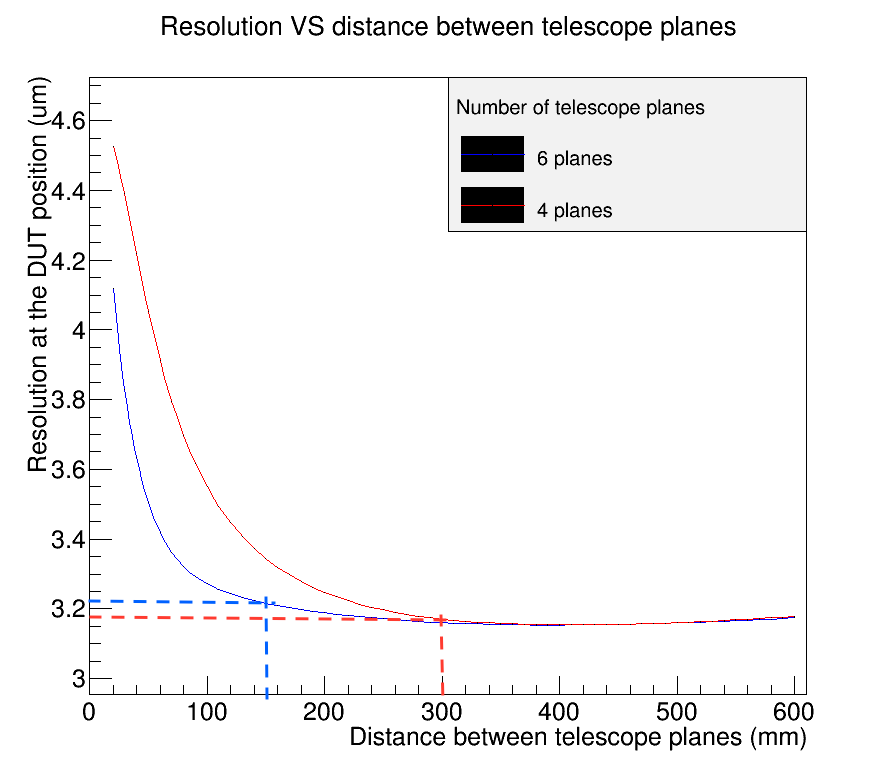
\includegraphics[width = 0.7\textwidth]{Pictures/X0/resolution_4Vs6planes_4-7GeV.png}
      \caption{Estimation of the resolution measured at the DUT position as a function of the distance between two telescope planes of the same arm.
      The blue lines is the results for six planes, whereas the red line is for four planes. 
      The dashed lines are the maximal distance between two planes due to the rail limitation of the telescope frame.}
      \label{fig:estimationRes4.7GeV}
    \end{figure}

    \begin{figure}
      %\centering
      \missingfigure{Mechanics}
    \end{figure}

    \subsection{experimental set-up}

    \begin{itemize}
      \item beam structure
      \item telescope
      \item Fan
    \end{itemize}
    \begin{figure}
      %\centering
      \missingfigure{Picture of telescope and PLUME}
    \end{figure}

    \subsection{Software analysis}

    Due to the specific acquisition which was done with EUDAQ, the analysis was a bit complicated.
    EUTelescope was coded to expect six telescope planes plus a single DUT.
    One way to overcome this problem was to perform a biased analysis.
    Instead of performing the alignment of the telescopes and then the DUT for an analysis, this step has to be done in one way.
    Nevertheless, the alignment procedure was not working.

    To perform the alignment, I have used a python script written by Claus Kleinwort, which reads the hit position of every sensor and use GBL and MP-II to perform the alignment.

